%\documentclass[sigplan,screen,review,noacm]{acmart}
\documentclass[sigplan,screen,noacm]{acmart}

\usepackage{subcaption}

\copyrightyear{2023}
\acmYear{2023}
% \acmDOI{XXXXXXX.XXXXXXX}

%% These commands are for a PROCEEDINGS abstract or paper.
\acmConference[Preprint]{TBD}{Mrach,
  2023}{Charlottesville, VA}

\acmBooktitle{Technical Report University of Virginia, Biocomplexity Institute, March, 2023, Charlottesville, VA, U.S.A., in preparation for 2023 OLCF User Meeting,
October 17-18, 2023, Registration by Sept 11.} 

\newcommand{\refBooktitle}{{\bf Reference:}\\ Nate Kimball, Wes Brewer, Gregor von Laszewski, and Geoffrey
C. Fox. 2023. OSMI Benchmark. In Technical Report University of Virginia, Biocomplexity Institute, March, 2023, Charlottesville, VA, U.S.A., in preparation for 2023 OLCF User Meeting,
October 17-18, 2023, Registration by Sept 11.}
\acmPrice{15.00}
\acmISBN{978-1-4503-XXXX-X/18/06}

%%%%%%%%%%%%%%%%%%%%%%%%%%%%%%%%%%%%%%%%%%%%%%%%
%
% REMOVE ACM PAPER INFO
%
\setcopyright{none}
\settopmatter{printacmref=False} % Removes citation information below abstract
\renewcommand\footnotetextcopyrightpermission[1]{} % removes footnote with conference information in first column
\pagestyle{plain}
%%%%%%%%%%%%%%%%%%%%%%%%%%%%%%%%%%%%%%%%%%%%%%%%


\begin{document}

\title{Towards the OSMI Benchmark with Cloudmesh Experiment Executor to support the FAIR principle}


\author{Nate Kimball}
\affiliation{%
  \institution{University of Virginia}
  \streetaddress{Biocomplexity Institute\\
                Town Center Four\\
                994 Research Park Boulevard}
  \city{Charlottesville}
  \state{VA}
  \postcode{22911}
  \country{USA}
}

\author{Wes Brewer}
\affiliation{%
  \institution{Oak Ridge National Laboratory}
  \streetaddress{1 Bethel Valley Road}
  \city{Oak Ridge}
  \state{TN}
  \postcode{37830}
  \country{USA}}
\email{brewerwh@ornl.gov}

\author{Gregor von Laszewski}
\email{laszewski@gmail.com}
\orcid{0000-0001-9558-179X}
\affiliation{%
  \institution{University of Virginia}
  \streetaddress{Biocomplexity Institute\\
                Town Center Four\\
                994 Research Park Boulevard}
  \city{Charlottesville}
  \state{VA}
  \postcode{22911}
  \country{USA}
}

\author{Geoffrey C. Fox}
\email{gcfexchange@gmail.com}
\affiliation{%
  \institution{University of Virginia}
  \streetaddress{Biocomplexity Institute\\
                Town Center Four\\
                994 Research Park Boulevard}
  \city{Charlottesville}
  \state{VA}
  \postcode{22911}
  \country{USA}
}


% \renewcommand{\shortauthors}{Trovato and Tobin, et al.}

%%
%% The abstract is a short summary of the work to be presented in the
%% article.
\begin{abstract}
We explore the relationship between certain network configurations and the performance of distributed Machine Learning systems. We build upon the Open Surrogate Model Inference (OSMI) Benchmark, a distributed inference benchmark for analyzing the performance of machine-learned surrogate models developed by Wes Brewer et. Al. We focus on analyzing distributed machine-learning systems, via machine-learned surrogate models, across varied hardware environments. By deploying the OSMI Benchmark on platforms like Rivanna HPC, WSL, and Ubuntu, we offer a comprehensive study of system performance under different configurations. The paper presents insights into optimizing distributed machine learning systems, enhancing their scalability and efficiency. We also develope a framework for automating the OSMI benchmark. 

  TODO: fix CCSXML, ccsdec
\end{abstract}

\begin{CCSXML}
<ccs2012>
   <concept>
       <concept_id>10002951.10003227.10003241.10003244</concept_id>
       <concept_desc>Information systems~Data analytics</concept_desc>
       <concept_significance>500</concept_significance>
       </concept>
   <concept>
       <concept_id>10010520.10010521.10010537.10003100</concept_id>
       <concept_desc>Computer systems organization~Cloud computing</concept_desc>
       <concept_significance>500</concept_significance>
       </concept>
   <concept>
       <concept_id>10011007.10011006.10011072</concept_id>
       <concept_desc>Software and its engineering~Software libraries and repositories</concept_desc>
       <concept_significance>500</concept_significance>
       </concept>
 </ccs2012>
\end{CCSXML}

\ccsdesc[500]{Information systems~Data analytics}
\ccsdesc[500]{Computer systems organization~Cloud computing}
\ccsdesc[500]{Software and its engineering~Software libraries and repositories}


% up to 5 keywords
\keywords{benchmark, deep learning, mlcommons}

\received{March 2023}
%\received[revised]{12 March 2009}
%\received[accepted]{5 June 2009}

 %%%%%%%%%%%%%%%%%%%%%%%%%%%%%%%%%%%%%%%%%%%%%%%%
% next line can be removed if submitted to acm
\settopmatter{printfolios=true}
%%%%%%%%%%%%%%%%%%%%%%%%%%%%%%%%%%%%%%%%%%%%%%%%

\maketitle

\refBooktitle

\section{Introduction}

With the proliferation of machine learning as a tool for science, the need for efficient and scalable systems is paramount. This paper explores the Open Surrogate Model Inference (OSMI) Benchmark, a tool for testing the performance of machine-learning systems via machine-learned surrogate models. The OSMI Benchmark, originally created by Wes Brewer and colleagues, serves to evaluate various configurations and their impact on system performance.

Our research pivots around the deployment and analysis of the OSMI Benchmark across various hardware platforms, including the high-performance computing (HPC) system Rivanna, Windows Subsystem for Linux (WSL), and Ubuntu environments. 

In each experiment, there are a variable number of TensorFlow model server instances, overseen by a HAProxy load balancer that distributes inference requests among the servers. Each server instance operates on a dedicated GPU, choosing between the V100 or A100 GPUs available on Rivanna. This setup mirrors real-world scenarios where load balancing is crucial for system efficiency.

On the client side, we initiate a variable number of concurrent clients executing the OSMI benchmark to simulate different levels of system load and analyze the corresponding inference throughput.

On top of the original OSMI-Bench, we implemented an object-oriented interface in Python for running experiments with ease, streamlining the process of benchmarking and analysis. The experiments rely on custom-built images based on NVIDIA's tensorflow image. The code works on several hardwares, assuming the proper images are built. 

Additionally, We develop a script for launching simultaneous experiments with permutations of pre-defined parameters with Cloudmesh Experiment-Executor. The Experiment Executor is a tool that automates the generation and execution of experiment variations with different parameters. This automation is crucial for conducting tests across a spectrum of scenarios.

Finally, we analyze the inference throughput and total time for each experiment. By graphing and examining these results, we draw critical insights into the performance dynamics of distributed machine learning systems. 

In summary, this paper offers a comprehensive examination of the OSMI Benchmark in diverse distributed ML systems. We aim to contribute to the optimization of these systems, by providing a framework for finding the best performant system configuration for a given use case. Our findings pave the way for more efficient and scalable distributed computing environments.

\section{OSMI}

The Open Surrogate Model Inference (OSMI) Benchmark is a distributed inference benchmark for analyzing the performance of machine-learned surrogate models and is described in its original form as "smiBench" in "Production Deployment of Machine-Learned Rotorcraft Surrogate Models on HPC" [1]. In this paper, the authors explore how to optimally deploy several different types of machine-learned surrogate models used in rotorcraft aerodynamics on HPC. The authors developed three machine learning models at three different sizes, including Long Short Term Memory (LSTM), Convolutional Neural Network (CNN), and Temporal Convolutional Neural Network (TCNN) models with 2M, 44M, and 212M trainable parameters, respectively. The surrogate models are trained on random data because the main purpose of this benchmark is to test deployment efficiency. The models are tested on a wide range of configurations to study optimal deployment scenarios. The paper explores several parameters that affect inference, including batch size, number of requests, network protocol, server, GPU, number of GPUs, and concurrency.              

\section{Benchmark}

\subsection{Hardware}

\paragraph{WSL.} - Nate

I use Ubuntu 20.04.5 LTS on WSL2. My laptop is a dell XPS 15 with an Intel(R) Iris(R) Xe GPU.

\paragraph{Ubuntu.} - Gregor

\paragraph{Rivanna.} - Nate

On Rivanna, we experiment with V100 and A100 gpus. There were many obstacles to overcome in the Rivanna implementation. Due to memory constraints, we had to reduce the number of requests sent per experiment to 16,384 unlike the original paper that used 32,768 for most of their analysis. We reduced the maximum batch size in our experiments to 128 as well. We ran into the problem of jobs running on the same machine overlapping in ports, so we implemented an algorithm that produce unique port numbers for each program based on the parameters. In some of the experiments we ran, A ValueError occurred for unknown reasons. These errors disappeared when those specific experiments were reran.


\subsection{Hardware used for this Research}

The benchmarks we present in the next sections have been run on a number of compute resources. This includes not only an HPC at the University of Virginia (UVA) but also a desktop, a laptop, and Google Colab to represent different classes of computing resources that students have access to. We used the following resources:

\begin{itemize}
\item {\bf Rivanna}~\citep{www-rivanna} -- The Rivanna HPC cluster is  a system hosted at the University of Virginia with 15 different  hardware configurations spanning 575 nodes.  There exist 5 different  classes of GPUs on these nodes. The Rivanna HPC follows the  condominium model and continues to receive additions of nodes and  upgrades at various times.
\item {\bf Google Colab}~\cite{google-colab} is a free-to-use interactive computing service offered by Google that provides on-demand access to GPUs and TPUs. Google Colab is designed to be used with machine learning and data analysis \cite{google-colab}. When running with Google Colab, multiple hardware configurations may be provided depending on the instance type. The Pro+ plan allocates an NVIDIA V100 with 53GB of RAM for a GPU configuration. The free  plan only offers 32 GB and a P100 GPU.
\item {\bf Desktop} -- A custom-built desktop with an AMD 5950X processor, 128GB memory, and fast NVMe storage.
\item {\bf Laptop} -- A store-bought laptop with an AMD 5900HX processor, 16GB memory, and NVMe storage.

\end{itemize}


The details of the machines are showcased in Table~\ref{tab:hwoverview}.

\begin{comment}
\begin{table*}[htb]
\begin{verbatim}
17 * servers with 8 a100 80G, 128 AMD EPYC 7742 CPU, 2T Memory, 100Gb Infiniband
 2 * servers with 8 a100 40G, 128 AMD EPYC 7742 CPU, 1T Memory, 100Gb Infiniband
15 * servers with 8 a6000, 48 AMD EPYC 7352 CPU, 250G Memory, 100Gb Infiniband
 2 * servers with 10 rtx2080, 40 Intel(R) Xeon(R) Gold 6148 CPU @ 2.40GHz, 376G Memory, 100Gb Infiniband
 5 * servers with 4 rtx3090, 32 AMD EPYC 7302 CPU 125G Memory, 100Gb Infiniband
12 * servers with 4 v100, 40 Intel(R) Xeon(R) Gold 6148 CPU @ 2.40GHz, 376G Memory, 100Gb Infiniband
 3 * servers with 4 v100, 36 Intel(R) Xeon(R) Gold 6240 CPU @ 2.60GHz, 376G Memory, 100Gb Infiniband
 1 * servers with 4 v100, 28 Intel(R) Xeon(R) Gold 6132 CPU @ 2.60GHz, 187G Memory, 100Gb Infiniband
\end{verbatim}
\end{table*}
\end{comment}


\begin{table*}[htb]
    \caption{Overview of the computing resources.}
    \label{tab:hwoverview}
    \begin{center}
    {\footnotesize
    \begin{tabular}{|l|r|r|r|r|r|r|r|r|}
        \hline
            {\bf Machine}  & {\bf Cores} & {\bf Memory} & {\bf GPU} & {\bf GPU}   &   {\bf Memory} & {\bf \# GPUs} & {\bf \# Nodes}  & {\bf Commissioned} \\ 
                     &  {\bf / Node} & {\bf / Node}  &  & {\bf Total} & {\bf / GPU} & {\bf / Node}     &   {\bf / Node}        &  \\
        \hline
        \hline
        Rivanna (UVA)    & 128 & 2000GB   & 136 & A100 & 80GB &  8  & 17 & Feb 2022 \\
                        & 128 & 1000GB   & 16 & A100 & 40GB &  8  &  2 & Jun 2022  \\  & 48 & 250GB   & 120 & A6000 & 48GB &  8  &  15 & Jun 2022  \\   
                        & 28  & 255GB    & 64 & K80  & 11GB &  8  &  8 & Jun 2018         \\
                        & 28  & 255GB    & 16 & P100 & 12GB &  4  &  4 & Jan 2018         \\
                        & 28  & 188GB    & 4 & V100 & 16GB &  4  &  1 & Feb 2019          \\
                        & 40  & 384GB    & 48 & V100 & 32GB &  4  & 12 & Feb 2021          \\
                        & 36  & 384GB    & 12 & V100 & 32GB &  4  &  3 & Apr 2022          \\
                        &  64 & 128     & 20 & RTX3090   & 24GB    & 4   &  5 & Feb 2023         \\
                        & 40  & 384GB    & 20 & RTX2080TI & 11GB & 10  &  2 & May 2021 \\                        
         \hline
         Google Colab      & -   & 32GB      & & P100      & 16GB    & 1 & - & March 2022 \\
         Google Colab Pro+ & -   & 53GB      & & V100      & 32GB    & 1 & - & March 2022 \\
         \hline
         Desktop 5950X     &  32 & 128GB     & 1& RTX3090   & 24GB    & 1 & 1 & Feb 2022   \\
         \hline
    \end{tabular}
    }
    \end{center}
\end{table*}

\paragraph{Filesystem Comparision}

We provide here the comparison of the file system that is motivated by observations made in \cite{???}.


TODO: include table



\subsection{Results}

\begin{figure*}[h]

\begin{minipage}[t]{0.4\textwidth}
  \centering
  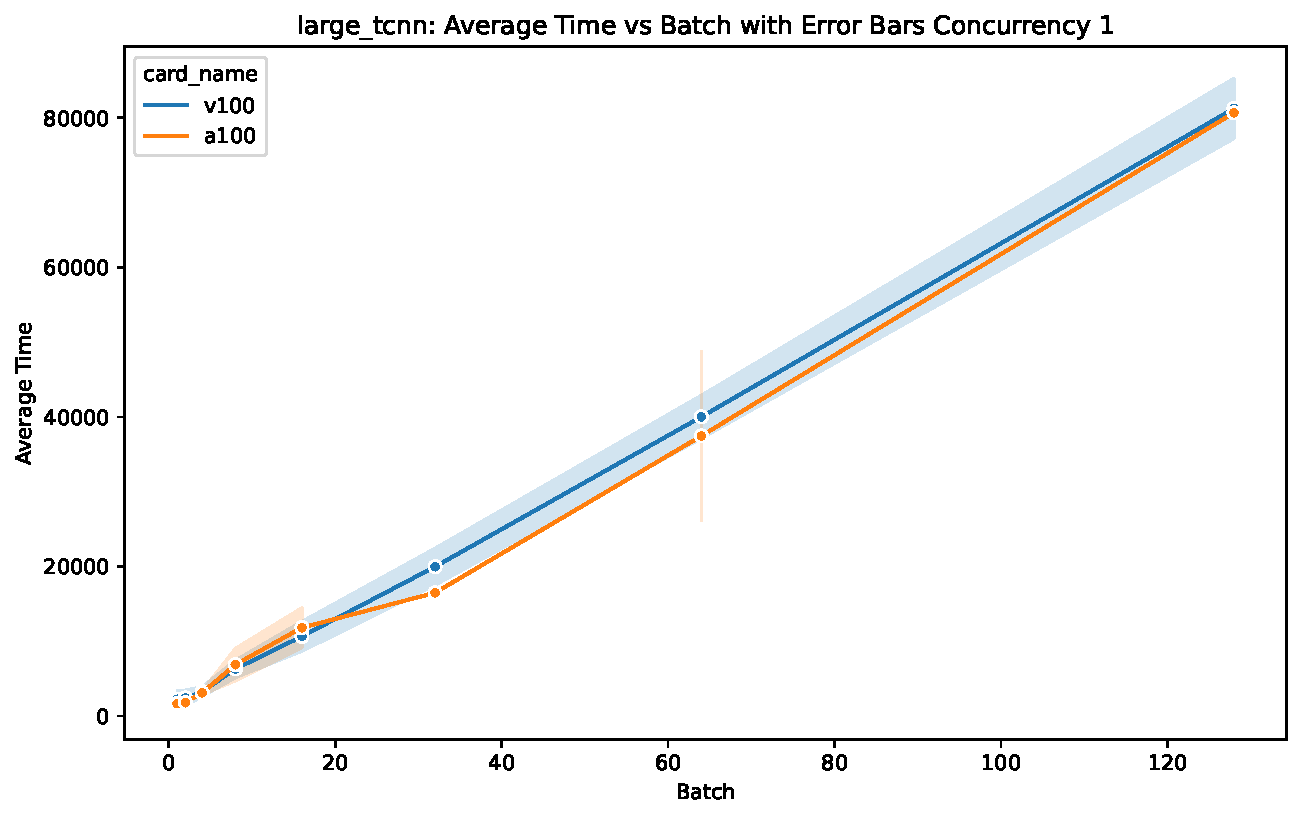
\includegraphics[width=1.0\linewidth]{images/time_vs_batch_large_tcnn_1.pdf}
  \caption{Time vs batch size for the large tcnn model}
    \label{fig:time-batch-large}
  \Description{Time vs batch size for the large tcnn model}

  \centering
  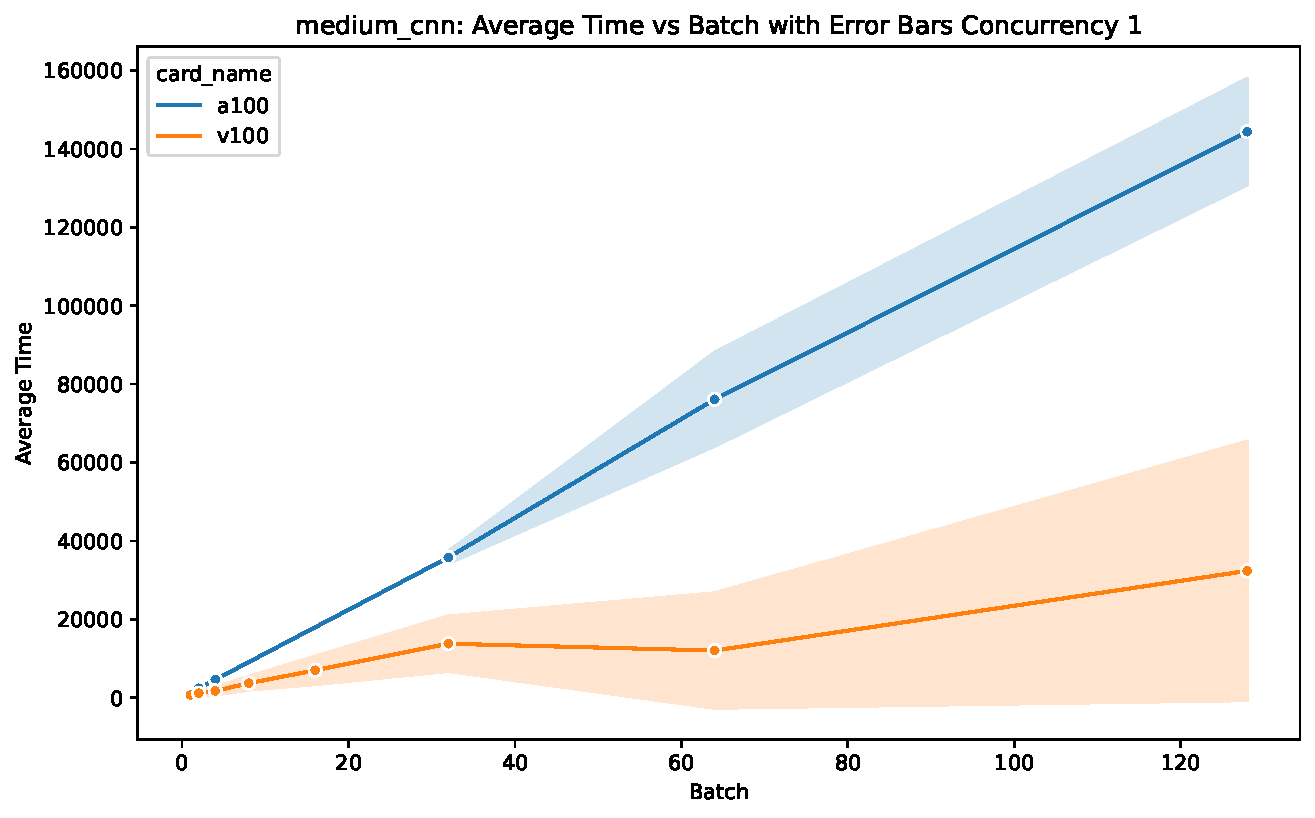
\includegraphics[width=1.0\linewidth]{images/time_vs_batch_medium_cnn_1.pdf}
  \caption{Time vs batch size for the medium tcnn model}
    \label{fig:time-batch-medium}
  \Description{Time vs batch size for the medium tcnn model}

  \centering
  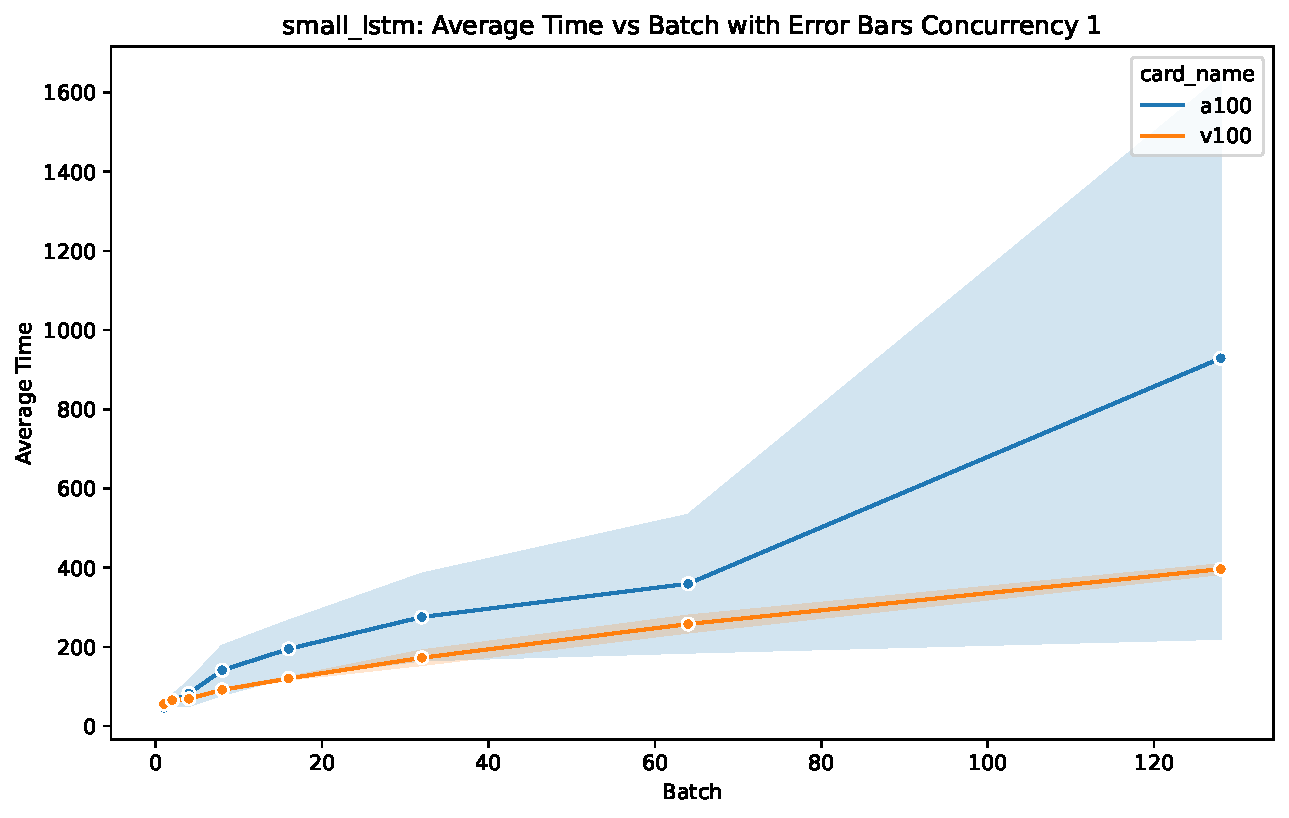
\includegraphics[width=1.0\linewidth]{images/time_vs_batch_small_lstm_1.pdf}
  \caption{Time vs batch size for the small lstm model}
    \label{fig:result-4}
  \Description{Time vs batch size for the small lstm model}
\end{minipage}
\ \
\begin{minipage}[t]{0.4\textwidth}
  \centering
  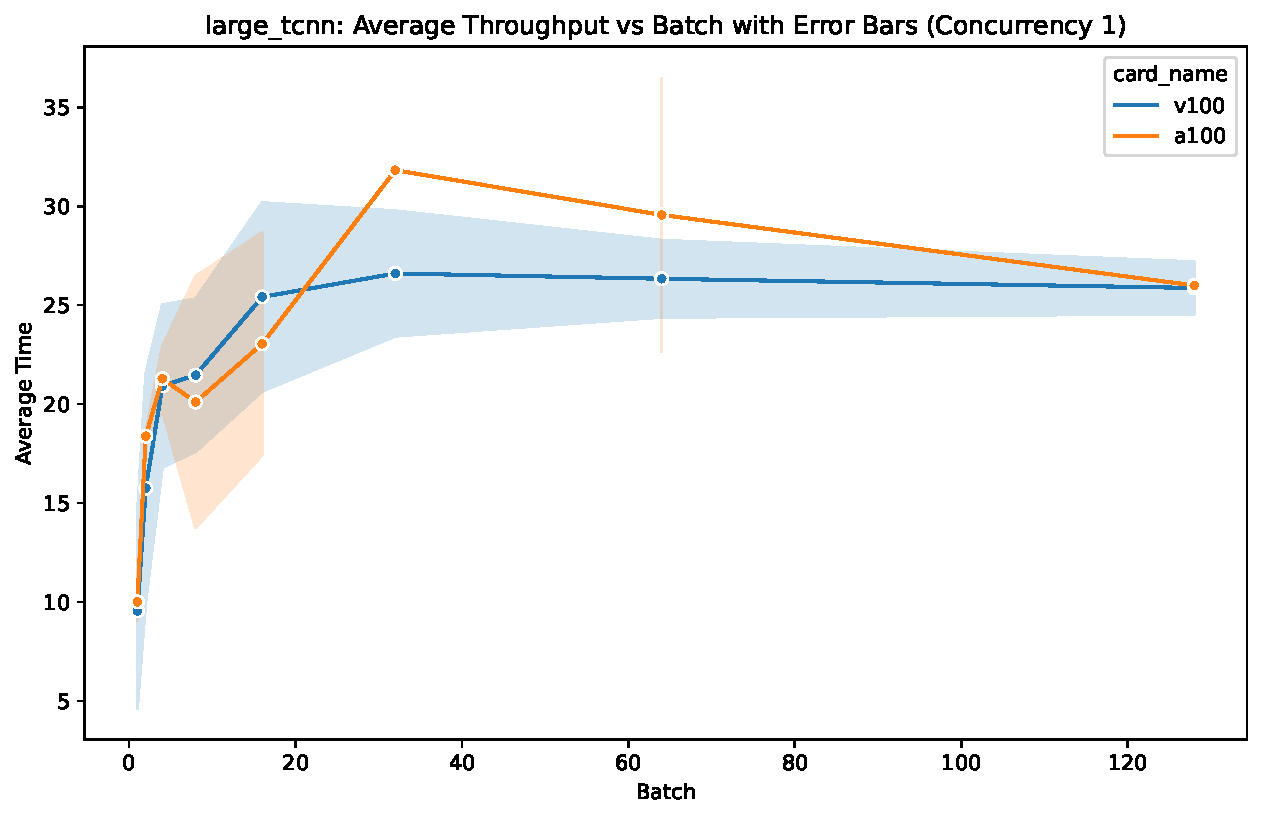
\includegraphics[width=1.0\linewidth]{images/throughput_vs_batch_large_tcnn_1.pdf}
  \caption{Throughput vs batch size for the large tcnn model}
    \label{fig:result-5}
  \Description{Throughput vs batch size for the large tcnn model}

  \centering
  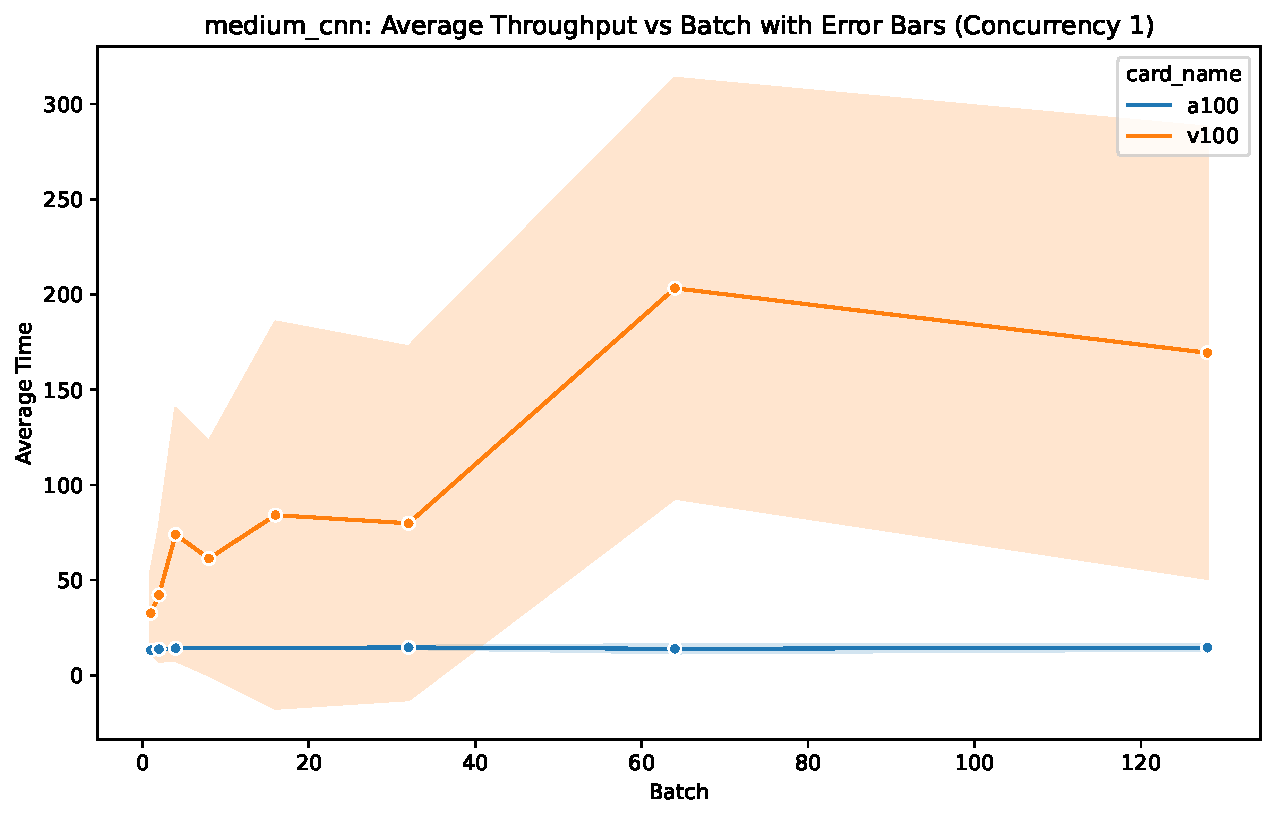
\includegraphics[width=1.0\linewidth]{images/throughput_vs_batch_medium_cnn_1.pdf}
  \caption{Throughput vs batch size for the large cnn model}
    \label{fig:result-6}
  \Description{Throughput vs batch size for the large cnn model}

  \centering
  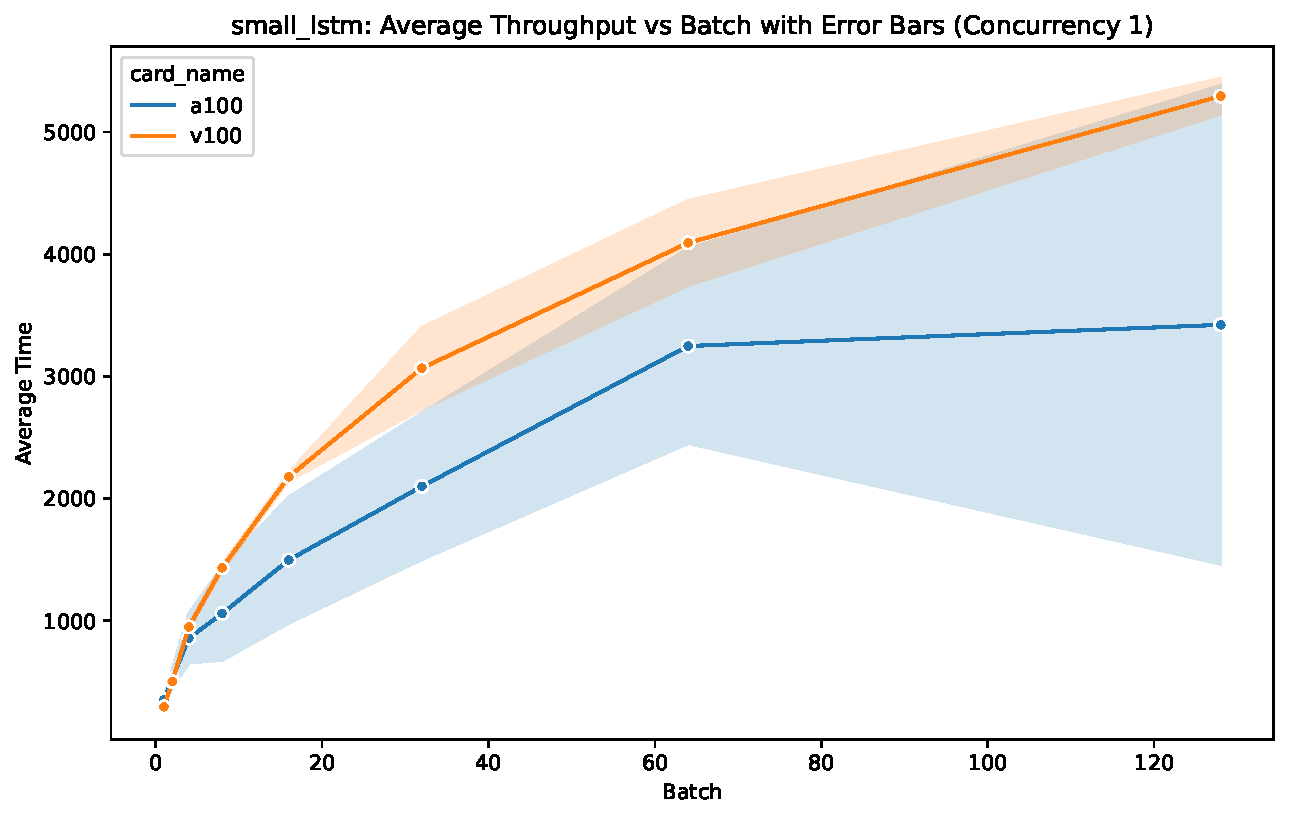
\includegraphics[width=1.0\linewidth]{images/throughput_vs_batch_small_lstm_1.pdf}
  \caption{Throughput vs batch size for the small lstm model}
    \label{fig:result-3}
  \Description{Throughput vs batch size for the small lstm model}

\end{minipage}
\end{figure*}















% Figure \ref{fig:throughput-vs-gpus} is a recreation of Wes Brewer et al. Production Deployment of Machine-Learned Rotorcraft Surrogate Models on HPC Fig. 7. Weak scaling analysis of TF Serving (with gRPC and HAProxy) inference performance on Summit for three rotorcraft surrogate models.
Figure \ref{fig:throughput-vs-gpus} is a recreation of Wes Brewer et al. Production Deployment of Machine-Learned Rotorcraft Surrogate Models on HPC Fig. 6. T2NI benchmark results using the medium Surf/CNN model with batch size 128. (use total time)

Figure \ref{fig:result-3} is a recreation of Fig. 4. Rotorcraft surrogate model embedded benchmarks using the Flask inference server with HTTP protocol, however, we use TensorFlow serving as our inference server.

\section{Examples Citation}

Example \cite{cloudmesh-hybrid-workflow}

%%%%%%%%%%%%%%%%%%%%%%%%%%%%%%%%%%%%%%%%%%%%%%%%%%%%%%%%%%%%%

\begin{acks}

We like to thank ...

TBD. DOE, NSF, NIST
To Robert, for the bagels and explaining CMYK and color spaces.
\end{acks}

%%%%%%%%%%%%%%%%%%%%%%%%%%%%%%%%%%%%%%%%%%%%%%%%%%%%%%%%%%%%%

\bibliographystyle{ACM-Reference-Format}
\bibliography{paper}

%%%%%%%%%%%%%%%%%%%%%%%%%%%%%%%%%%%%%%%%%%%%%%%%%%%%%%%%%%%%%
\appendix
%%%%%%%%%%%%%%%%%%%%%%%%%%%%%%%%%%%%%%%%%%%%%%%%%%%%%%%%%%%%%

\section{Online Resources}

\begin{description}

\item{Code}
\item{Cloudmesh-common}
\item{Cloudmesh-StopWatch}
\item{Mlcommons}

\end{description}

\end{document}

\endinput
%%
%% End of file `sample-sigplan.tex'.
